\documentclass{article}%

% Margins
\usepackage[top=1in, bottom=1in, left=1in, right=1in]{geometry}

% Fonts
\usepackage[T1]{fontenc}
\usepackage[utf8]{inputenc}

% Section formatting
\usepackage[center]{titlesec}

% Formatting
\usepackage{setspace}
\doublespacing
\usepackage{caption}
\hyphenation{con-sti-tu-tion-al}
\usepackage{amsmath}
\renewcommand\refname{VI. References}

% Media
\usepackage{graphicx}
\usepackage{wrapfig}
\usepackage{float}
\usepackage{booktabs}
\graphicspath{ {../figures/} }

% Table of Contents
\usepackage{tocloft}
\usepackage{etoolbox}

% List of Figures
\makeatletter
\renewcommand*\l@figure{\@dottedtocline{1}{0em}{7em}}
\makeatother

% Ensure dots in table of contents
\makeatletter
\renewcommand*\l@section{\@dottedtocline{1}{1.5em}{2.3em}}
\makeatother
% Rename table of contents
\renewcommand*\contentsname{\textbf{TABLE OF CONTENTS}}
% Rename list of figures
\renewcommand*\listfigurename{\textbf{LIST OF FIGURES}}

\begin{document}
\pagestyle{empty}
% Title
% \pagenumbering{roman}
\begin{center}
{\fontfamily{ptm}\Large\selectfont
    Novel Approach to Constructing an Ultra Low Cost Flowcell Biosensor\\
}
% 4 returns = ?? vspace
\vspace{1.7cm}
{\fontfamily{ptm}\large\selectfont
    THESIS\\
}
% 5 returns = ?? vspace
\vspace{2cm}
{\fontfamily{ptm}\large\selectfont
    Presented to the Faculty of the Department of Physics and Astronomy\\
    in Partial Fulfillment of the Major Requirements\\
    for the Degree of\\
}
% 6 returns = ?? vspace
\vspace{2.1cm}
{\fontfamily{ptm}\large\selectfont
    BACHELOR OF SCIENCE IN\\
    PHYSICS\\
}
% 6 returns = ?? vspace
\vspace{2cm}
{\fontfamily{ptm}\selectfont
    \large{Jeffery Summers}\\
}
% 6 returns = ?? vspace
\vspace{1.6cm}
{\fontfamily{ptm}\selectfont
    \large{May 2019}\\
}
% 6 returns = ?? vspace
\vspace{2cm}
{\fontfamily{ptm}\selectfont
    \copyright 2019 Middle Tennessee State University\\
    All rights reserved.\\
}
\vspace{0.2cm}
{\fontfamily{ptm}\small\selectfont
    The author hereby grants to MTSU permission to reproduce\\
    and to distribute publicly paper and electronic\\
    copies of this thesis document in whole or in part\\
    in any medium now known or hereafter created.\\
}
\end{center}
\pagenumbering{roman}

\pagebreak

% Signature page
% Number pages with lowercase roman numerals
\begin{center}
{\fontfamily{ptm}\selectfont
    Novel Approach to Constructing an Ultra Low Cost Flowcell Biosensor\\
}
% 3 returns = ?? vspace
\vspace{1.8cm}

{\fontfamily{ptm}\selectfont
Jeffery Summers
}
% 18 returns = ?? vspace
\vspace{8cm}
\end{center}
% Author signature
\begin{flushleft}
    {\fontfamily{ptm}\selectfont
    Signature of Author:\\
    }
\end{flushleft}
\vspace{0cm}
\hrule
\begin{flushright}
    {\fontfamily{ptm}\small\selectfont
    Department of Physics \& Astronomy\\
    May 2019\\
    }
\end{flushright}
\vspace{1.5cm}
% Thesis supervisor signature
\begin{flushleft}
    {\fontfamily{ptm}\selectfont
    Certified by:\\
    }
\end{flushleft}
\vspace{0cm}
\hrule
\begin{flushright}
    {\fontfamily{ptm}\small\selectfont
    Dr. William Robertson\\
    Department of Physics \& Astronomy\\
    Thesis Supervisor\\
    }
\end{flushright}
\vspace{1.5cm}
% Department chair signature
\begin{flushleft}
    {\fontfamily{ptm}\selectfont
    Accepted by:\\
    }
\end{flushleft}
\vspace{0cm}
\hrule
\begin{flushright}
    {\fontfamily{ptm}\small\selectfont
    Dr. Ronald Henderson\\
    Professor of Physics \& Astronomy\\
    Chair, Physics \& Astronomy\\
    }
\end{flushright}
\vspace{1.5cm}

\pagestyle{plain}
\pagebreak

% Abstract
\section*{ABSTRACT}
\addcontentsline{toc}{section}{\hspace{0.34in}Abstract}
Here's my abstract, gee how interesting.\\
\pagebreak

% Table of Contents
\tableofcontents
\pagebreak

% List of Figures
\listoffigures
\pagebreak

% Introduction
\fontfamily{ptm}\selectfont
\pagenumbering{arabic}
\section*{I. INTRODUCTION}
\addcontentsline{toc}{section}{I.\hspace{0.25in}Introduction}
\begin{flushleft}
	\hspace{0.5in}
	Flowcell sensors have many applications; disease detection, measuring refractive index and reactivity to name a few. These sensors have been operating on the basis of electromagnetic surface phenomena for decades. Most flowcells on the market work by exploiting surface plasma oscillations (SPOs). These oscillations are highly sensitive to changes in the optical properties of the adjacent medium and it follows from Maxwell's equations when the dielectric functions of each medium satisfies \cite{JLTROB:1}
	
	\[
    	\frac{\epsilon_{spo}}{\epsilon_{adjacent}} < -1
	\]
	\hspace{0.5in}
	Metals like aluminum, copper, gold, and silver have negative dielectric functions at wavelengths in the red/infrared, so films of these metals are used as to generate SPOs in most flowcell sensors via a process known as Surface Plasmon Resonance (SPR). An SPR system utilizes light-prism coupling to excite the surface electrons on a thin metal film deposited on the hypotenusal face of the prism. There are quite a few drawbacks for using metal films, however. Metals are highly reactive so each time an SPR system is used a new prism must be used. These films also require particular wavelengths of incident light to excite the oscillations. Rather than using metal films, one-dimensional photonic crystals, or multilayers, can be designed to exhibit the phenomenon of surface electromagnetic waves (SEWs) or Bloch surface waves (BSWs), named after the physicist Felix Bloch who was famous for working with periodic systems. These surface waves have the same practical application as SPOs. Multilayers overcome both of the shortcomings of metal films listed here. They can be designed to work for any wavelength and are typically made of nonreactive glass. In addition to these benefits, we expect that our 3-D printed and multilayer-based flowcell sensor will be more sensitive and precise with its measurements and be far cheaper to both build and maintain compared to traditional SPR sensors.

	\hspace{0.5in}
	To take measurements with our sensor we look at the reflected image of incident laser light. Our multilayer is designed to trap incident light in the last layer at a special angle; this results in a dark band in our reflected image. A diagram of the process is shown below.
	
	\hspace{0.5in}
	As fluids or gases are put into the flowcell chamber the index of refraction, $n_c$, changes. The condition for total internal reflection, found from Snell's law, for the interface between a glass prism and some transmitting medium whose index of refraction varies with time is given by:
	\[
			\sin{\theta_c} = \frac{n_t(t)}{n_g}
	\]

	We obtain an expression for the angle of reflection as a function of time by the Law of Reflection:

	\[
			\theta_r(t) = \arcsin{\frac{n_t(t)}{n_g}}
	\]

	\hspace{0.5in}
	Note that this expression is for a single interface and hence does not accurately reflect our setup as we have a glass prism and a multilayer. With that said, this expression for $\theta_r$ does capture the essence of our setup; the reflected angle is a function of the index of refraction of the transmission. Using this fact we can associate variations in the flowcell chamber's index of refraction with differences in the angle of reflectance. These angular differences can be calculated by tracking the variation in the position of the dark band in the reflected image.

	\hspace{0.5in}
	Now with an an expression for the rate of change of reflected angle we can measure the index of refraction inside the flowcell chamber over time. From this data we can interpolate the mutual reactivity between molecules in a reaction, or maybe the rate of mixing of sugar water at a given temperature.

	\pagestyle{empty}
\end{flushleft}

\pagebreak

% Experimental Setup
\section*{\textbf{II. Experimental Design}}
\addcontentsline{toc}{section}{II.\hspace{0.15in} Experimental Design}

\begin{wrapfigure}{R}{2in}
    \includegraphics[width=2in]{multilayer.png}
    \caption{An illustration of the photonic crystal used in our sensor}
    \label{fig:multilayer}
\end{wrapfigure}
\hspace{0.15in}
The process of design for this experiment relies heavily on the use of a 15 milimeter right prism and our photonic crystal. The photonic crystal is composed of 3 bilayers of TiO2 and SiO2. The dielectric function of TiO2 is taken as $\epsilon_{TiO2} = 4.84 + 0.0007i$ and the dielectric function of SiO2 is taken as $\epsilon_{SiO2} = 2.1316 + 0.0001i$. It should be noted that the imaginary parts of each dielectric function may not be accurate due to the values being not well known and have been included to introduce some form of loss that fits the results of prior experiments. Figure 3 illustrates the structure of the multilayer.


The sensor is composed of three different parts: the primary stage, two beams, and the flowcell stage.  One of the two beams holds our laser and a focusing lens while the other holds the CCD and captures the reflected beam. Normally the laser light is too intense to pick up the surface mode in the reflected image. We attach a neutral density filter (d=3.5, see Figure \ref{fig:beams}) to the CCD to reduce the intensity and this allows us to image the surface mode. 

% Picture of beams, central stage, and flowcell stage
\begin{figure}[h]
    \begin{center}
    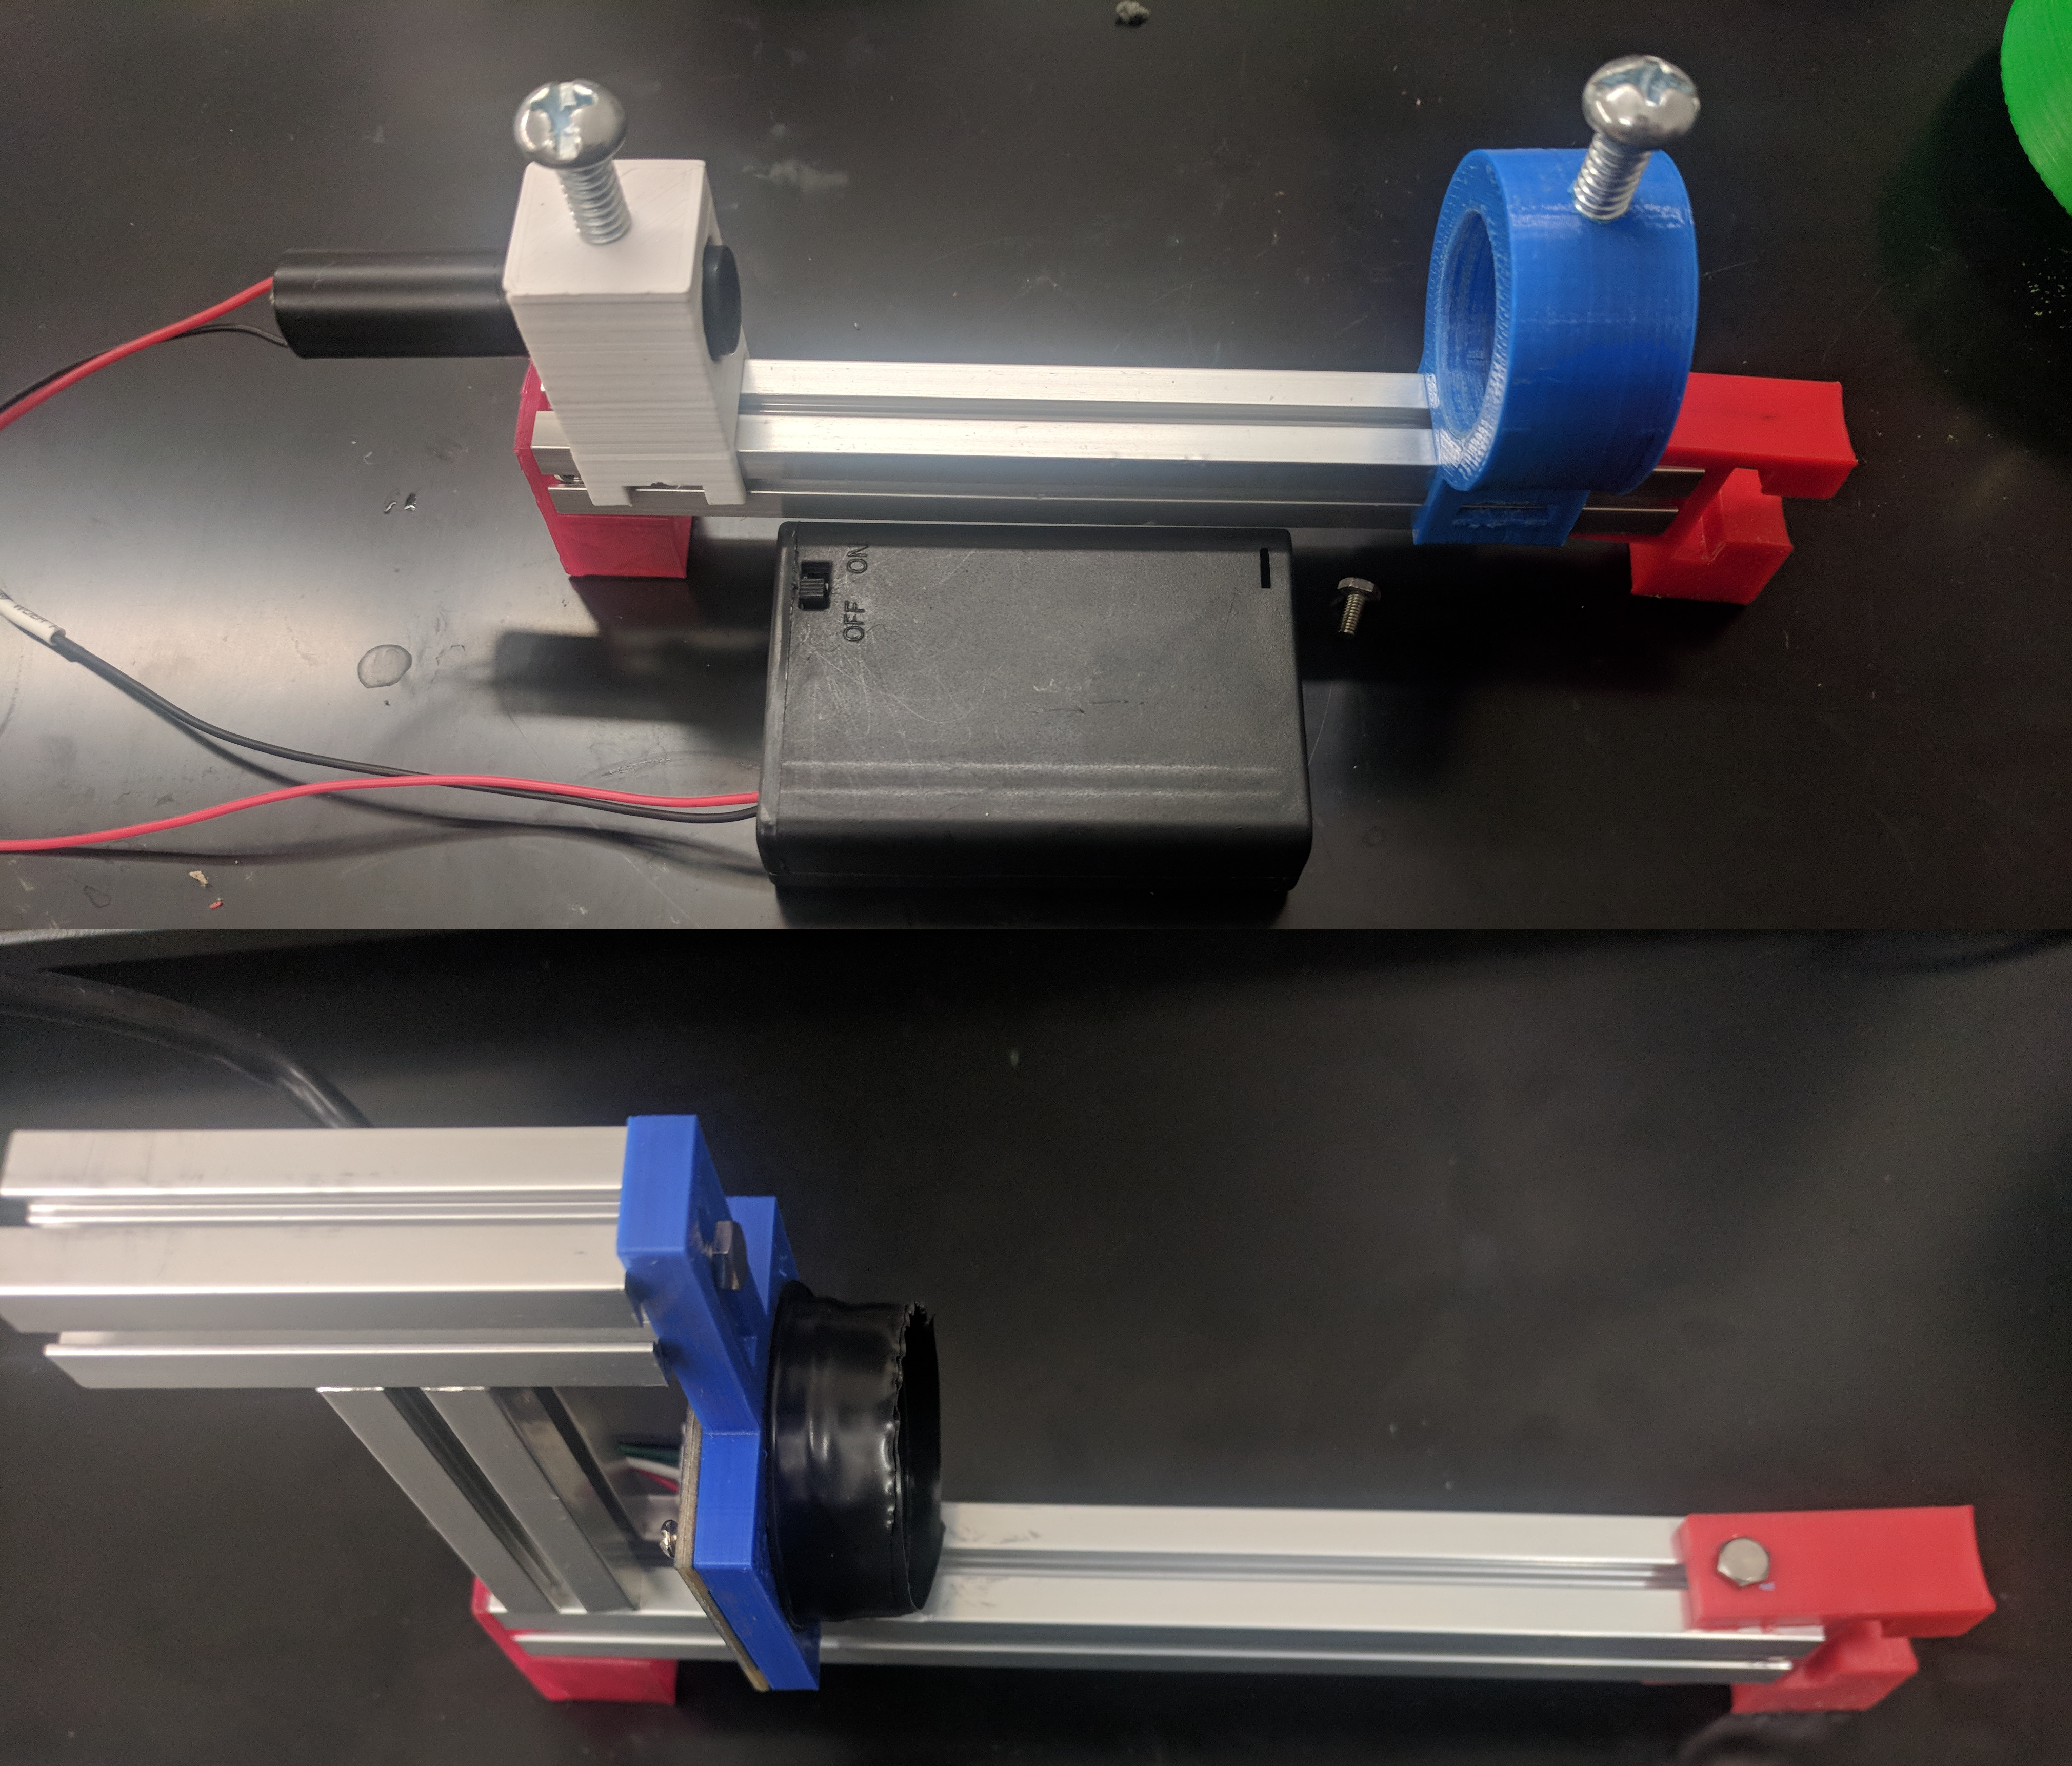
\includegraphics[width=0.6\textwidth]{arms.png}
    \caption{Top: the beam holding the laser and focusing lens. Bottom: the beam holding the camera and neutral density filter.}
    \label{fig:beams}
    \end{center}
\end{figure}

Each beam is a 15cm x 10mm x 10mm aluminum MakerBeam. Attached on the left side of each beam in Figure \ref{fig:beams} is a foot used to keep the beams level with the central platform. On the right side of each beam is a 3D printed connector used to attach the beams to the primary stage. The beams are capable of rotating around the axis that keeps these connectors in place, allowing a larger range of coupling angles for the laser-multilayer system.


The primary stage (see the green 3D printed fixture in Figure \ref{fig:centralstage}) acts as the center about which the incident beam can be coupled to the prism and then reflected onto the CCD. The design of this stage allows different types of multilayers to be used since the incident laser can be oriented at nearly any angle. The flowcell stage (see the blue 3D printed piece bolted into the primary stage in Figure \ref{fig:centralstage}) is a modular piece that is attached to the primary stage with four bolts. The prism, multilayer, and flowcell chamber are all strapped together on this stage via two pairs of 3D printed braces and hex screws. The modular nature of this piece of the sensor is valuable since multiple designs can be used to achieve the generate BSWs and it only takes between 40 minutes to an hour to print off each flowcell stage.

\begin{figure}[h]
\begin{center}
    \includegraphics[width=0.7\textwidth]{central_stage.png}
    \caption{Primary stage and flowcell stage of our sensor. The green round 3D printed fixture underneath the flowcell is the primary stage which the two beams are attached to via a small divot in the back. The blue 3D printed piece mounted to the primary stage is the flowcell stage. The glass prism, multilayer, and flowcell chamber are attached atop the flowcell stage with the use of hex screws and 3D printed braces.}
    \label{fig:centralstage}
\end{center}
\end{figure}


To flow liquids through the chamber the whole fixture must be water tight. To accomplish this we designed the flowcell so that a rubber gasket could be fit around the chamber. When the braces are tightened there is no liquid loss at the interface during operation, however the chamber is made of PLA and liquid will leak through the plastic after a few hours. The two apertures on top of the flowcell are used for inflow and outflow. To ensure no leaks occur when flushing the chamber we wrapped each aperture with electrical tape before attaching our tubing. 

\begin{figure}[h]
\begin{center}
    \includegraphics[width=0.7\textwidth]{flowcell.jpg}
    \caption{The flowcell stage, prism, multilayer and flowcell chamber. A rubber gasket is set in a groove around the chamber so that when the braces are tightened the interface between the multilayer and flowcell is liquid tight.}
    \label{fig:flowcellstage}
\end{center}
\end{figure}

The decision to print a flowcell stage separate from the primary stage allows the design to be tinkered with without wasting too much time. Using our 3D printers the primary stage takes about nine hours to print, while the flowcell stage only takes about fourty minutes to one hour. This is useful because the position of the glass prism (used to couple incident light to the multilayer) can be more conveniently oriented to produce BSWs. A diagram illustrating the coupling angle required for our multilayer is illustrated in Figure \ref{fig:couplingangle}. From that diagram it is easy to see how awkward an angle is needed for the sensor to operate, but the ability to translate the prism's bed by printing off another flowcell stage makes it natural to orient the laser at the coupling angle. The next section details how the coupling angle is computed and how data is collected by imaging the surface mode.

\begin{figure}[t!]
\begin{center}
    \includegraphics[width=\textwidth]{couplingangle.png}
    \caption{The geometry behind our coupling angle when the flowcell chamber is filled with water. The lines normal to the left leg and hypotenuse of the triangle represent the surface normals of the prism. The line $40^\circ$ from the left leg surface normal and $66^\circ$ from the hypotenusal surface normal represent the path of the incident light. The laser needs to be oriented about $5^\circ$ off of parallel with the hypotenusal face of our prism. It is quite an awkward angle, but a different flowcell stage can be printed to make reaching this coupling angle more natural by translating the prism's bed upward.}
    \label{fig:couplingangle}
\end{center}
\end{figure}
\pagebreak

% Methods
\section*{III. Methods}
\addcontentsline{toc}{section}{III.\hspace{0.12in}Methods}
\hspace{0.5in}
To collect data from our biosensor we first prepare the flowcell chamber with the correct substrate or liquid that acts as our reference point for measuring changes in optical properties. After the chamber is prepared we then turn on the beam and rotate it until the special angle is reached. 

\begin{wrapfigure}{L}{6cm}
    \includegraphics[width=6cm]{reflectivity_dip.png}
\end{wrapfigure}

This is quite a precise angle so we orient the beam near the the mode $\sim 63^{\circ}$ from the prism's surface normal for a chamber filled with water or air using our multilayer stack as seen in ??. This plot was generated from a Python program that I wrote which use a transfer matrix method to generate reflection and transmission amplitudes for a multilayer stack like the one we use in our experiment. To confirm the light has coupled to the surface mode we check the reflected image of the beam for a dark vertical band as seen in ??.

\begin{wrapfigure}{R}{6cm}
	\includegraphics[width=6cm]{darkband.png}
\end{wrapfigure}

As the index of refraction inside the flowcell chamber changes the dark band will translate left or right in our reflected image, depending on whether the index is increasing or decreasing. The shift in location of the band, in pixels, corresponds to an angular shift in the part of the reflected beam giving rise to the dark band. This is shown clearly in ?? as we see that a change from an index of 1.00 (air) to 1.33 (water) corresponds to an angular shift  of about $3^\circ$.


To test our sensor, we first fill the flowcell with water and then inject different concentrations watered down ethanol, isopropal alcohol, and acetone. The table below lists the indices of refraction for all of these liquids.
\begin{center}
\begin{tabular}{| c | c c c c c |}
	\hline
    {}      			& Ethanol & Isopropal Alcohol & Acetone & Water \\
	\hline
	Index of Refraction & 1.361   & 1.3772            & 1.3588  & 1.333 \\
    \hline
\end{tabular}
\end{center}

\pagebreak

% Results
\section*{IV. RESULTS}
\label{sec:results}
\addcontentsline{toc}{section}{IV. \hspace{0.05in} Results}
\hspace{0.25in}
The table in Figure \ref{fig:ethshift} lists the mixtures of ethanol used to test for a change in index of refraction. The plot below shows the different indices of refraction corresponding to mixture A being injected over the interval $[25, 55]$. Similarly mixture B was injected over the interval $[70, 90]$, and mixture C over $[100, 150]$. After the mixtures have time to settle in the chamber, they are flushed out with the same deionized water used to indicate the baseline mode position. Upon injecting a mixture with a higher index into the chamber we notice that the mode position shifts, as expected. 

\begin{wrapfigure}{R}{4in}
\hskip+1.7cm\begin{tabular}{| c c c c |}
	\hline
	Mixtures      	 & A     			  & B      			   & C \\
	\hline
	Ethanol (ml)  	 & 10.\underline{0}   & 20.\underline{0}   & 30.\underline{0} \\
	Water   (ml)  	 & 100.\underline{0}  & 100.\underline{0}  & 100.\underline{0} \\
	Index         	 & 1.338\underline{0} & 1.341\underline{8} & 1.345\underline{0} \\
	Pixel Shift  	 & 80.\underline{0}	  & 135.\underline{0}  & 245.\underline{0} \\
	Change in Index  & 0.004\underline{9} & 0.005\underline{2} & 0.011\underline{9} \\   
	\hline
\end{tabular}
	\includegraphics[width=4in]{annotated_mode_4-1-2019}
	\caption{Index shift measurements for ethanol.}
	\label{fig:ethshift}
\end{wrapfigure}

\hspace{0.1in}
Using this data we can acquire a value of an index shift per pixel shift to quantify the sensitivity of the sensor. All of the mixtures used for testing have indices between 1.3380 and 1.3464, meaning that when the pixel shift of each mixture is plotted against the index of each we should expect a linear graph (see Figure \ref{fig:modevsindex}) since small variations in reflected angle will yield a proportional shift in pixels.
By extrapolating the data provided in the figure below we that a shift in one pixel corresponds to a shift of about 0.0018 in index of refraction. This level of sensitivty the exceeds the necessary sensitive to detect surface loading \cite{roberstonpaper}.

\begin{figure}
\hskip+1.7cm\begin{tabular}{| c c c c |}
		\hline
		Mixtures      	 & A     			  & B      			   & C \\
		\hline
		Acetone (ml)  	 & 10.\underline{0}   & 20.\underline{0}   & 30.\underline{0} \\
		Water   (ml)  	 & 100.\underline{0}  & 100.\underline{0}  & 100.\underline{0} \\
		Index         	 & 1.338\underline{4} & 1.343\underline{0} & 1.346\underline{4} \\
		Pixel Shift  	 & 111.\underline{5}  & 206.\underline{0}  & 292.\underline{5} \\
		Change in Index  & 0.005\underline{2} & 0.009\underline{8} & 0.013\underline{2} \\   
		\hline
	\end{tabular}
	\newline
		\includegraphics[width=4in]{annotated_acetone_mode.png}
		\caption{\small{Index shift measurements for acetone.}}
\end{figure}
\vspace{-1.2cm}
\begin{figure}
\hskip+1.7cm\begin{tabular}{| c c c c |}
		\hline
		Mixtures      	 & A     			  & B      			   & C \\
		\hline
		70\% Isop Alc. (ml)  	 & 10.\underline{0}   & 20.\underline{0}   & 30.\underline{0} \\
		Water   (ml)  	 & 100.\underline{0}  & 100.\underline{0}  & 100.\underline{0} \\
		Index         	 & 1.339\underline{8} & 1.341\underline{2} & 1.344\underline{7} \\
		Pixel Shift  	 & 84.\underline{5}	  & 164.\underline{5}  & 223.\underline{0} \\
		Change in Index  & 0.006\underline{6} & 0.008\underline{0} & 0.011\underline{5} \\   
		\hline
	\end{tabular}
	\newline
		\includegraphics[width=4in]{annotated_isopropal_mode.png}
		\caption{\small{Index shift measurements for 70\% isopropyl alcohol.}}
\end{figure}
\pagebreak

% Conclusion
\section*{\textbf{V. CONCLUSION}}
\addcontentsline{toc}{section}{V.\hspace{0.18in}Conclusion}
\hspace{0.25in}
In conclusion, this is a fine alternative to traditional flowcell sensors on the market. The only parts that need to be bought are the multilayers, a low power laser, a focusing lens, and a CCD. The rest of the parts can be 3D printed. The sensor does have a few issues, however. The flowcell itself is not quite water tight. This could be solved by either machining the flowcell or coating the chamber with a water tight sealant. Some multilayers may have coupling angles that are awkward to reach with the current design, however the modular nature of the flowcell stage can aid in reaching the coupling angle. In addition to modifying the flowcell stage, a hemispherical prism could be used in place of the right triangular prism used in our aparatus. The largest uncertainty of our device comes from the error in our ability to measure the pixel shift of the surface mode. At the moment a nine by nine gaussian blur is used to smooth out the image of the surface mode leaving us with an uncertainty in the mode position of about $\pm 9$ pixel .

% Bibliography
\bibliography{references}
\bibliographystyle{ieeetr}
\addcontentsline{toc}{section}{VI.\hspace{0.13in}References}

\end{document}